\section{Simulation Setup, Results, and Discussion}
\label{sec:experiments}
\subsection{Tasks and Evaluation Protocol}
The evaluation preserves the fixed completion time, assigned endpoints, footprint, and physical limits across methods. The original 30 tasks comprise crossing, passage, and obstacle-field families, with five difficulty levels and two layouts per level. Crossing teams grow from three to seven UAVs; the other families use five UAVs. The square passage opening decreases from 4.4 to 2.8 m, and the four-obstacle size multiplier increases from 0.50 to 1.10. The workspace is $[-15,15]^2\times[0.5,7.5]$ m, and every main-benchmark flight lasts 12 s.

Additional physical tasks use a smaller $[-8,8]^2\times[0.5,7.5]$ m workspace. Crossing teams contain 10, 15, or 20 UAVs, with ten randomized start--goal realizations at each size. Passage and obstacle-field tasks use ten UAVs, three geometric levels, and five realizations per level. The passage openings are 3.2, 2.6, and 2.0 m; obstacle dimensions increase across levels. These 60 tasks change physical congestion while retaining the nominal corridor-growth limits. A separate targeted passage study considers teams of five, eight, and ten UAVs at a 16 s horizon. The accompanying data provide the task definitions and outcomes.

The principal methods are \textbf{LIOM (proposed)}, with a hard-QP entry and the complete recovery loop; \textbf{Soft LIOM}, which starts directly with the relaxed loop; \textbf{Hard box--iterative}, which imposes exact kinematics and zero relative-box slack while retaining reconstruction; \textbf{Hard RSC--iterative}, which uses exact kinematics and separating half-spaces with the same reconstruction opportunities; and \textbf{Hard box--once}, which solves only the initial hard-box QP. One-shot RSC and one-shot soft variants provide further ablations. All share the reference policy, spatial construction, safe pair screening, physical acceptance, and total budget. These task-matched hard and soft corridor variants examine the iterative mechanisms associated with~\cite{bu2025,li2022liom,park2021} in the same UAV model.

The archived comparisons use a 1 s hard-entry allowance. Section 7.7 evaluates 1, 3, and 5 s allowances and establishes the recommended 3 s setting for new runs. The main comparison has three repetitions per scene and method, with rotated method order; additional one-shot variants have one repetition. The repetitions characterize runtime variability. Paired case records identify whether a method returns an accepted motion within the budget. CPU time includes MATLAB and the OSQP worker; wall time includes reference generation, construction, numerical assembly, solver setup and exchange, solution, reconstruction, and verification. Process startup and plotting are excluded. All attempts, including failures, enter runtime summaries. The 30 s budget is a nominal stopping rule checked between stages. The results distinguish accepted motions returned within 30 s, accepted motions returned later, and attempts without an accepted motion.

\subsection{Physical, Numerical, and Implementation Settings}
The UAV is a generic hovering-capable multirotor with a spherical planning radius of 0.25 m and required surface clearance of 0.10 m. The translational limits are 4 m/s and 3 m/s$^2$. These values define a moderate flight envelope for the planning and tracking studies. The main grid has $K=60$ intervals. Table~\ref{tab:settings} gives the common numerical settings.
\begin{table}[htbp]
\begin{adjustwidth}{-\extralength}{0cm}
\caption{Common settings. Linear-row tolerances use the corresponding native SI units. Final acceptance retains the physical tolerances below.\label{tab:settings}}
\small\begin{tabularx}{\fulllength}{lYlY}\toprule
Parameter & Value & Parameter & Value\\\midrule
$T_f$ / $K$ & 12 s / 60 & $w_a$ & 0.05\\
$r$ / $c$ & 0.25 / 0.10 m & $v_{\max}$ / $a_{\max}$ & 4 m/s / 3 m/s$^2$\\
$\ell_s$ / $\ell_r$ & 1.5 / 1.2 m & Expansion increment & 0.15 m\\
$\rho_q^{(0)}$, $\rho_s^{(0)}$ & $10^3$ & Penalty caps / growth & $10^5$ / 2\\
$\varepsilon_q$ / $h_0$ & $10^{-3}/300$ m$^2$ / 0.2 s & $\varepsilon_s$ & $10^{-4}$ m\\
Candidate row tolerance & $10^{-3}$ & OSQP absolute / relative tolerance & $10^{-6}$ / $10^{-6}$\\
Maximum outer rounds & 12 & Hard entry / regular solve & 1 / 5 s (archived runs)\\
Nominal planning budget & 30 s & Geometric guard & $10^{-5}$ m\\
Clearance tolerance & $2\times10^{-5}$ m & Speed tolerance & $2\times10^{-5}$ m/s\\
Acceleration tolerance & $2\times10^{-5}$ m/s$^2$ & Endpoint / integration tolerance & $10^{-9}$ m, $10^{-9}$ m/s\\
\bottomrule\end{tabularx}
\end{adjustwidth}\end{table}

Sparse QPs are assembled numerically in MATLAB R2021b and solved by OSQP~\cite{stellato2020osqp}. The computer uses an Intel Core i9-12900H processor and 16 GB RAM. OSQP checks candidate readiness in blocks of 250 iterations, using the local linear-row tolerance and, for relaxed candidates, both recovery thresholds. Readiness permits reconstruction; complete-interval physical checking determines acceptance. An identical-matrix OSQP audit compares candidate-readiness stopping with ordinary solver termination at two numerical tolerances.

The initial penalty scale favors consistency while the cap limits conditioning problems. The defect threshold uses a five-UAV, 60-interval reference scale; its normalized form permits team and grid comparisons. The control-effort coefficient sets its relative importance in the augmented objective. Grouped sensitivity tests vary these choices around the development settings. The static guide grid is 0.65 m. SFM uses a 0.02 s integration step, a 2 m/s preferred speed, gains $A_p=A_o=4$ m/s$^2$, decay length 0.35 m, look-ahead 0.35 m, response time 0.3 s, and tangential factor 0.5. All remaining settings and the frozen scenario definitions accompany the experiment scripts.

The SFM samples form geometric polylines. Repeated points are removed, and arc-length interpolation evaluates~\eqref{eq:reference} on the 0.2 s optimization grid. The prescribed scalar law therefore determines geometric resampling onto the optimization grid. Initialization time includes SFM, guide construction, timing, and any guide fallback.

\subsection{Accepted Motion and Main-Benchmark Performance}
Complete-interval checks are applied to the integrated motion~\eqref{eq:arc}. Squared pair distance is quartic in interval time, so its extrema follow from a cubic derivative. Point-to-AABB distance is minimized over box-face crossing intervals and their stationary points. Workspace extrema, endpoints, and integration identities are checked as well. Speed is affine within each interval and acceleration is constant, allowing exact interval checks of their Euclidean limits. These tests examine every pair and obstacle, including pairs screened out of the QP.

Table~\ref{tab:main-new} reports computation over the main benchmark. Proposed LIOM has mean wall time 7.83 s, compared with 4.03 s for Hard RSC--iterative. The bounded hard entry can route an attempt to recovery before a longer hard solve would finish, so its runtime includes the cost of maintaining that option. The following winding tasks identify the specific local incompatibilities for which the additional route is useful. All task-level outcomes are retained with the timing records.

\begin{table}[htbp]
\begin{adjustwidth}{-\extralength}{0cm}
\caption{Computation on the 30-scene main benchmark with the original 1 s LIOM hard entry and three executions per method and scene. Means and the wall-time P95 include all 90 attempts, including budget stops. Rounds and QPs are mean counts.\label{tab:main-new}}
\centering\small
\begin{tabular}{lrrrrr}\toprule
Method & CPU (s) & Wall (s) & P95 (s) & Rounds & QPs\\\midrule
\textbf{LIOM (proposed)} & 8.66 & 7.83 & 25.39 & 2.08 & 2.46\\
Soft LIOM & 8.84 & 8.42 & 26.92 & 2.27 & 2.29\\
Hard box--iterative & 16.08 & 14.45 & 30.06 & 3.92 & 3.92\\
Hard RSC--iterative & 4.56 & 4.03 & 10.56 & 1.44 & 1.44\\
Hard box--once & 5.37 & 5.29 & 13.57 & 1.00 & 1.00\\
\bottomrule\end{tabular}
\end{adjustwidth}
\end{table}

\begin{table}[htbp]
\caption{Accepted proposed-method motions in the first main-benchmark repetition (29 scenes). Integration errors quantify numerical consistency. Clearance and motion limits are checked separately over complete intervals.\label{tab:verification-new}}
\centering\small
\begin{tabular}{lr}\toprule
Quantity & Observed extremum\\\midrule
Minimum inter-UAV center distance (m) & 1.388\\
Minimum obstacle surface clearance (m) & 0.4959\\
Maximum speed (m/s) & 3.325\\
Maximum acceleration (m/s$^2$) & 3\\
Maximum endpoint coordinate error (m) & 1.199e-14\\
Maximum integration-identity error & 8.882e-16\\
Maximum control correction (m/s$^2$) & 9.663e-05\\
Maximum coordinate displacement from QP nodes (m) & 0.01585\\
\bottomrule\end{tabular}
\end{table}

\begin{figure}[htbp]
\begin{adjustwidth}{-\extralength}{0cm}\centering
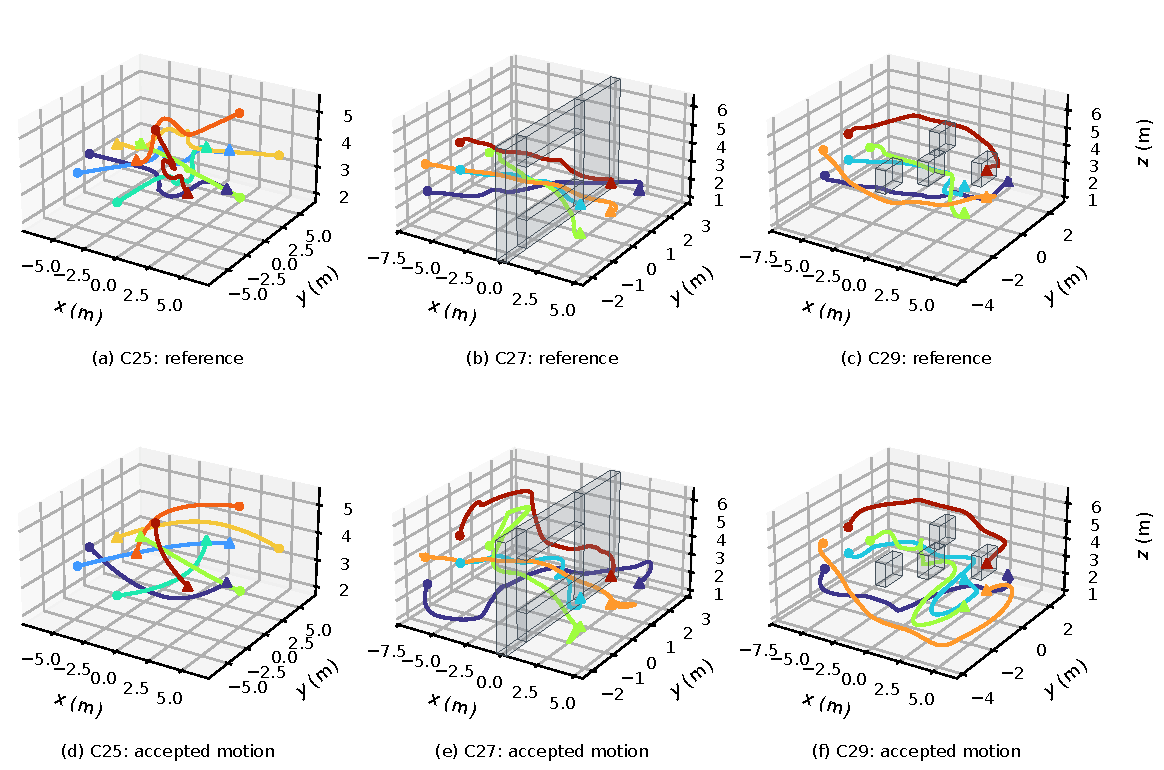
\includegraphics[width=\fulllength]{figures_revision/representative_motions.pdf}
\caption{Representative accepted cooperative motions with metric axes. Starts are circles, fixed goals are triangles, and colors identify UAVs. The full 30-scene overview is provided separately in the reproducibility package.\label{fig:scenes}}
\end{adjustwidth}\end{figure}
\begin{figure}[htbp]
\begin{adjustwidth}{-\extralength}{0cm}\centering
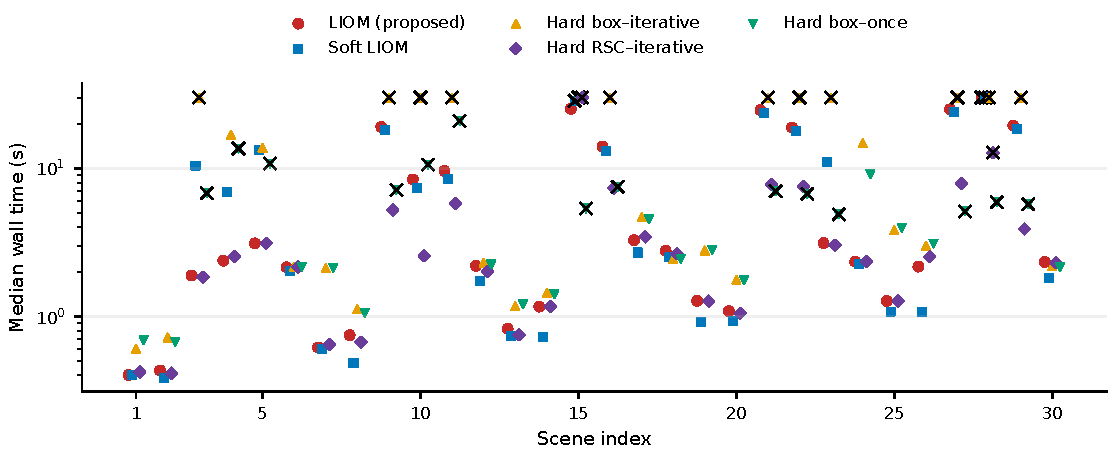
\includegraphics[width=\fulllength]{figures_revision/main_performance.pdf}
\caption{Main-benchmark computation. Per-scene median wall times use separated method positions and a logarithmic axis. Crosses mark a scene--method combination with an incomplete attempt among its three repetitions. All attempts enter the timing summaries.\label{fig:performance}}
\end{adjustwidth}\end{figure}

\begin{figure}[htbp]
\begin{adjustwidth}{-\extralength}{0cm}\centering
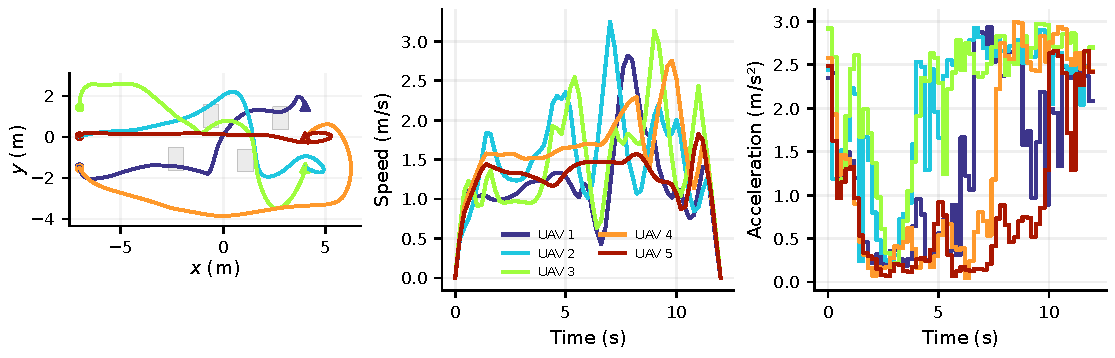
\includegraphics[width=\fulllength]{figures_revision/control_profiles.pdf}
\caption{Planar projection and individual UAV speed and acceleration histories for a representative accepted motion. Colors identify UAVs consistently across the panels.\label{fig:controls}}
\end{adjustwidth}\end{figure}

\subsection{Recovery in Winding Counterflow Tasks}
\label{sec:winding}
Three full-height walls with alternating openings produce repeated turns and opposing traffic. The representative task contains five UAVs, 2.2 m openings, and a fixed 24 s flight horizon with $h=0.2$ s. The spatial and relative growth limits, motion envelope, footprint, acceptance thresholds, and 30 s planning budget remain unchanged. A common 0.325 m static-guide grid resolves the openings. Each method receives the same saved reference and is charged the same measured initialization time. Hard RSC--iterative retains its reconstruction loop.

An exploratory search identified the task in Figure~\ref{fig:winding-recovery}. In the three initial paired executions of this task, proposed LIOM accepted the motion after five recovery rounds in 26.59--27.18 s. Soft LIOM also accepted all three executions, taking 25.33--25.72 s. Hard RSC--iterative completed eight reconstruction rounds per execution without acceptance within the budget. These repetitions characterize one physical task. Section~\ref{sec:external} reports a further paired execution alongside the nonlinear and sequential-convex methods. The accepted motion has minimum center separation 1.086 m, minimum obstacle surface clearance 0.495 m, maximum speed 3.577 m/s, and maximum acceleration 2.990 m/s$^2$; the respective requirements are 0.60 m, 0.10 m, 4 m/s, and 3 m/s$^2$.

An independent phase-I linear program minimizes a common row-scaled violation of the initial hard-RSC constraints. Its primal and dual objectives both equal 0.21915, with primal residual below $5\times10^{-14}$ and dual stationarity residual below $2\times10^{-17}$. Removing the relative rows alone, or the kinematic equalities alone, gives zero phase-I objective. These diagnostic checks identify an incompatibility between the selected relative restrictions and exact motion consistency. The complete returned motion satisfies both requirements after reconstruction. The diagnostic relaxations are used only to identify the conflict.

\begin{figure}[htbp]
\begin{adjustwidth}{-\extralength}{0cm}\centering
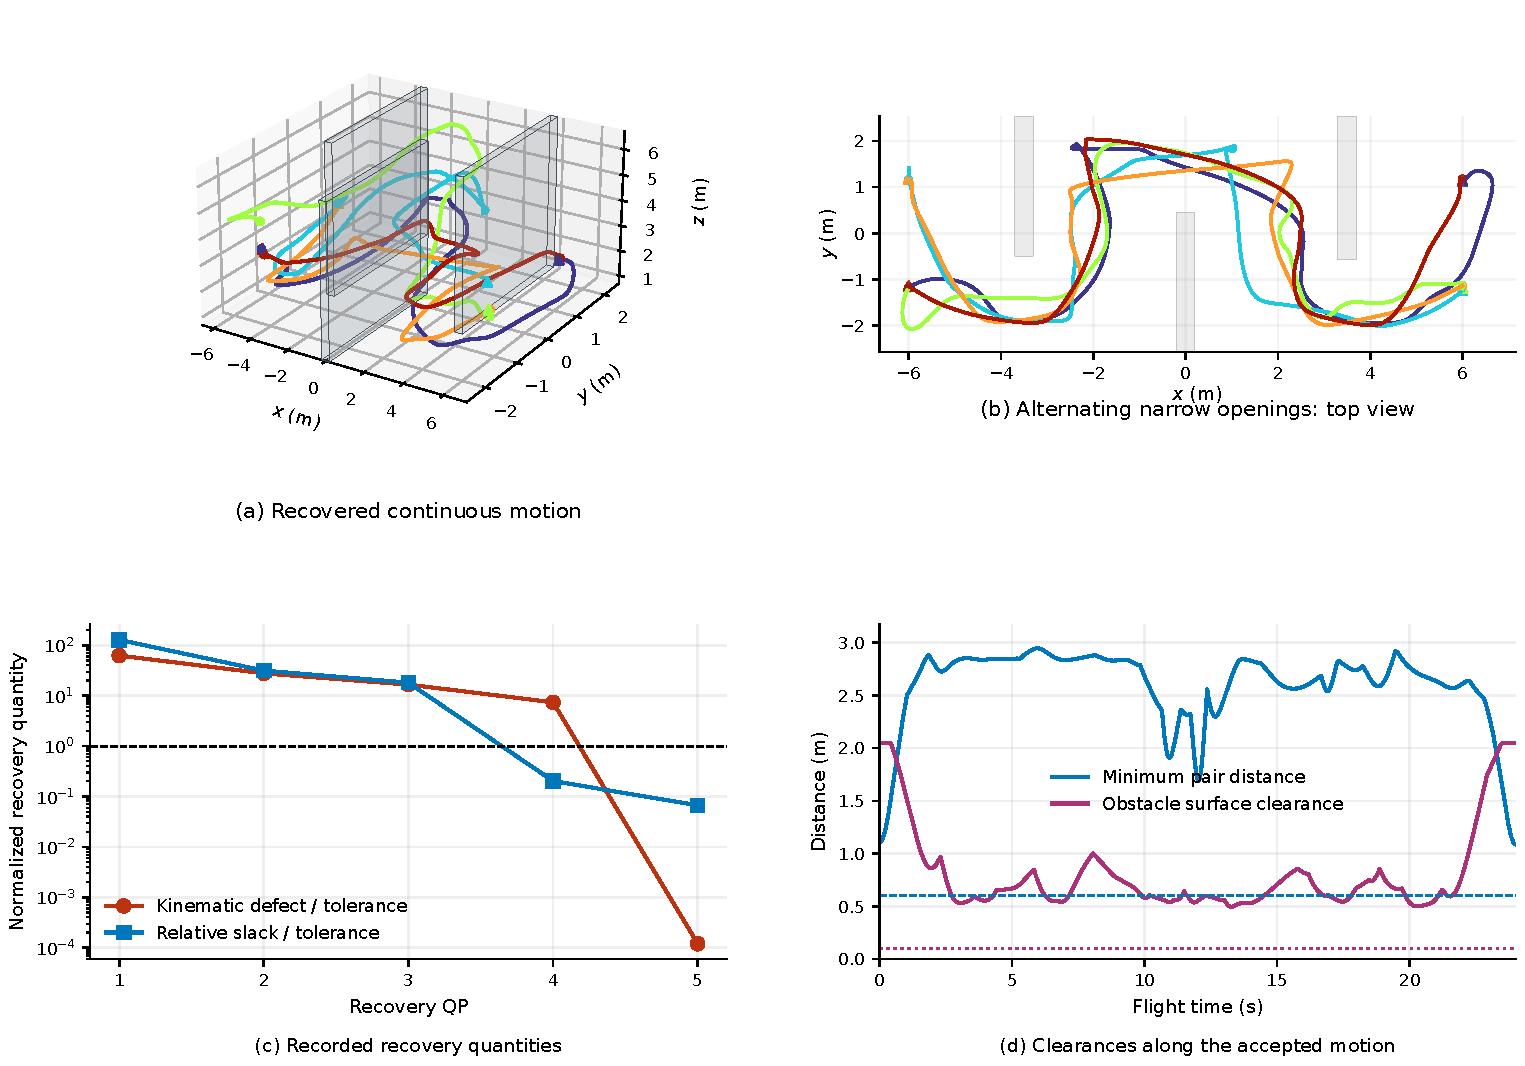
\includegraphics[width=\fulllength]{figures_revision/winding_recovery_case.pdf}
\caption{Recovery in a winding counterflow task. Colors identify UAVs. The recovery quantities are divided by their acceptance thresholds; the dashed unit line marks numerical recovery. The clearance curves visualize the integrated motion, whose acceptance is determined by complete-interval checks.\label{fig:winding-recovery}}
\end{adjustwidth}\end{figure}

A separate set of 12 previously untested random layouts contains a second recovered task whose initial hard QP has matching phase-I primal and dual objectives of 0.35420. The proposed method returns a checked motion for this task, while iterative hard RSC exhausts the common budget. This independently generated case supports the same conflict mechanism. The complete 12-layout outcomes and all exploratory records accompany the data.

Figure~\ref{fig:winding-map} varies physical opening width, team size, and prescribed flight time around the identified geometry. The nominal corridor-growth limits are unchanged. Both methods accept the three-UAV tasks. With five UAVs and 2.2 m openings, proposed LIOM additionally accepts the 24 s and 28 s tasks. Widening the openings permits both methods to succeed. The map locates the additional recovery region under physical congestion; it also shows where neither method returns an accepted motion within the common budget.
\begin{figure}[htbp]
\begin{adjustwidth}{-\extralength}{0cm}\centering
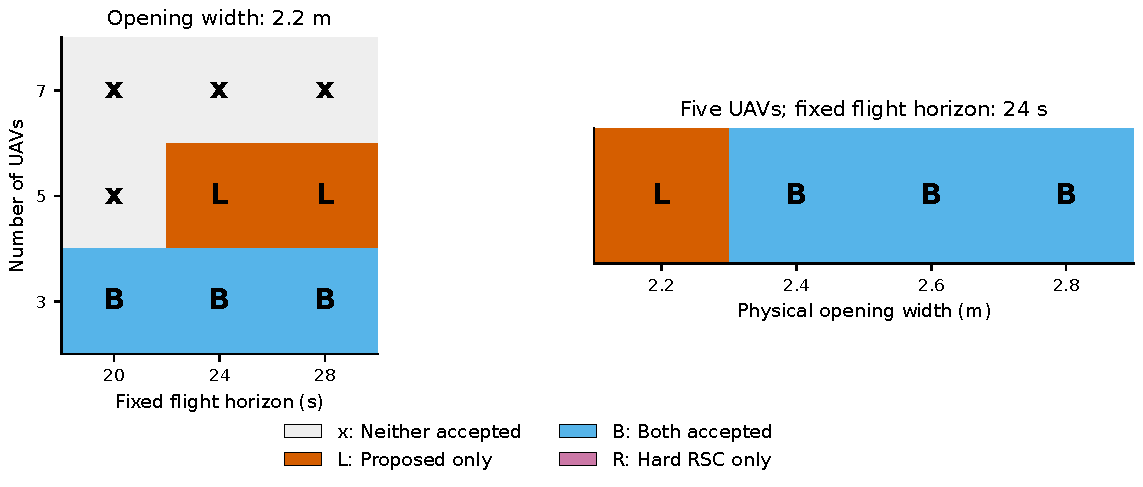
\includegraphics[width=\fulllength]{figures_revision/physical_recovery_map.pdf}
\caption{Exploratory physical-parameter map around the same winding layout. Letters supplement color: B, both accepted; L, proposed LIOM only; R, Hard RSC--iterative only; x, neither accepted. Twelve distinct settings are evaluated; the five-UAV, 24 s, 2.2 m setting appears in both panels. Every setting uses the same reference for both methods and the same 30 s budget.\label{fig:winding-map}}
\end{adjustwidth}\end{figure}


\subsection{Task-Matched Nonlinear and Sequential Convex Comparisons}
\label{sec:external}
Three additional strategies are adapted to the same UAV task. ASCO-3D~\cite{li2021asco} changes the active collision-risk range, retaining the preceding successful reference after a failed reduced solve. Direct NLP imposes all sampled collision restrictions simultaneously. SCP-3D~\cite{augugliaro2012} uses the distance-norm tangent restrictions of Eq.~(17) in~\cite{augugliaro2012}, with supporting planes for the static boxes. All use hard integration equations, the same polyhedral motion limits, fixed endpoints, fixed horizon, and control-effort objective. Collision restrictions are evaluated at quarter-interval arc samples with reachable-motion padding. The returned motion undergoes the same endpoint reconstruction and complete-interval acceptance tests as LIOM.

The nonlinear ASCO and direct-NLP instances use CasADi~\cite{andersson2019} and Ipopt~\cite{wachter2006} with the ma57 linear solver. Every quadratic subproblem uses OSQP. SCP assembles its sparse matrices directly; ASCO iterations without active nonlinear rows also use the QP backend. ASCO's original risk-range lengths are scaled by the ratio of UAV radius to the vehicle-disc radius in the source implementation. Its update rule and 50-round ceiling are retained; the common 30 s budget governs the comparison.

The paired study comprises six original benchmark tasks, both winding layouts, and 15- and 20-UAV tasks. The winding tasks use $T_f=24$ s and $K=120$; the remaining tasks use $T_f=12$ s and $K=60$. The methods are evaluated serially. Each method receives the identical saved reference and is charged its measured generation time. The comparison records one execution per task--method pair. The nonlinear baselines are rerun with ma57; the unchanged QP implementations retain their recorded measurements. Construction, solution, and final checking all enter the reported time, including calls that overrun the nominal stopping budget.

\begin{table}[htbp]
\begin{adjustwidth}{-\extralength}{0cm}
\caption{Task-matched planning times in seconds, including recorded initialization. LIOM uses the original 1 s hard entry in this comparison; the nonlinear columns are rerun with Ipopt/ma57. A cross denotes no accepted motion; $\dagger$ denotes an accepted motion returned after the nominal 30 s budget. Each entry is one recorded execution.\label{tab:external}}
\small\begin{tabularx}{\fulllength}{Ycrrrrr}\toprule
Task & $N$ & \textbf{LIOM (1 s)} & Hard RSC & ASCO-3D & Direct NLP & SCP-3D\\\midrule
C01 & 3 & \textbf{1.72} & 0.90 & 5.25 & 2.61 & 1.77\\
C03 & 5 & \textbf{1.51} & 1.42 & 3.50 & 29.05 & 3.27\\
C05 & 5 & \textbf{3.14} & 3.38 & 16.33 & 33.58$^{\dagger}$ & 5.47\\
C25 & 7 & \textbf{1.29} & 1.23 & 21.35 & 9.33 & 12.52\\
C27 & 5 & \textbf{24.35} & 7.55 & 8.61 & 27.79 & 5.41\\
C29 & 5 & \textbf{19.54} & 4.07 & 15.06 & 27.16 & 10.32\\
Winding A & 5 & \textbf{26.36} & 25.14 & $\times$\,33.72 & $\times$\,47.10 & $\times$\,28.41\\
Winding B & 5 & \textbf{31.92$^{\dagger}$} & $\times$\,30.07 & $\times$\,31.50 & $\times$\,31.36 & $\times$\,30.05\\
15-UAV & 15 & \textbf{27.49} & 29.97 & $\times$\,34.07 & 59.34$^{\dagger}$ & 19.91\\
20-UAV & 20 & \textbf{30.12$^{\dagger}$} & 27.70 & $\times$\,31.27 & $\times$\,106.75 & $\times$\,30.06\\
\bottomrule\end{tabularx}
\end{adjustwidth}\end{table}


Table~\ref{tab:external} reports the ma57 comparison. LIOM completes C01, C03, C05, and C25 in 1.29--3.14 s. In C27, LIOM returns an accepted motion in 24.35 s, while ASCO, hard RSC, and SCP complete the same task in 8.61, 7.55, and 5.41 s. The ma57 direct-NLP solve also accepts C27, in 27.79 s. These results show how the direct hard path and the recovery path distribute computation across tasks.

Winding A combines three alternating openings with opposing traffic. LIOM and iterative hard RSC return accepted motions in 26.36 and 25.14 s in this comparison. ASCO's candidate motions continue to fail collision checks when its budget is exhausted; SCP reports infeasibility for its initial tangent problem. The hard-RSC result supplements the earlier repetitions in Section~\ref{sec:winding}. The positive phase-I certificate identifies an incompatible initial local problem, and later reconstruction can reach a feasible corridor configuration. In Winding B, LIOM produces a physically accepted motion at 31.92 s; the ma57 baselines and the other hard comparisons return no accepted motion in their recorded attempts. The late LIOM output is marked explicitly in the table.

For the 15-UAV task, LIOM, hard RSC, and SCP complete in 27.49, 29.97, and 19.91 s. Direct NLP returns an accepted motion after its nominal budget, and ASCO ends without an accepted motion. At 20 UAVs, hard RSC completes in 27.70 s and LIOM returns an accepted motion at 30.12 s. Symbolic construction consumes the remaining budget in the two winding direct-NLP tasks and the 20-UAV direct-NLP task. The source records separate construction, numerical solution, and physical checking.



\subsection{Physical Congestion and Computational Scaling}
\label{sec:scaling}
The physical-congestion study varies crossing-team size, opening width, and obstacle dimensions while retaining the nominal corridor-growth limits. Figure~\ref{fig:physical} reports the mean computation in each group, including attempts that reach the stopping budget. The 30 s plateau marks termination at the nominal computational budget. These measurements characterize computational load, while the paired winding tasks provide direct evidence of recovery from incompatible local constraints.

\begin{figure}[htbp]
\begin{adjustwidth}{-\extralength}{0cm}\centering
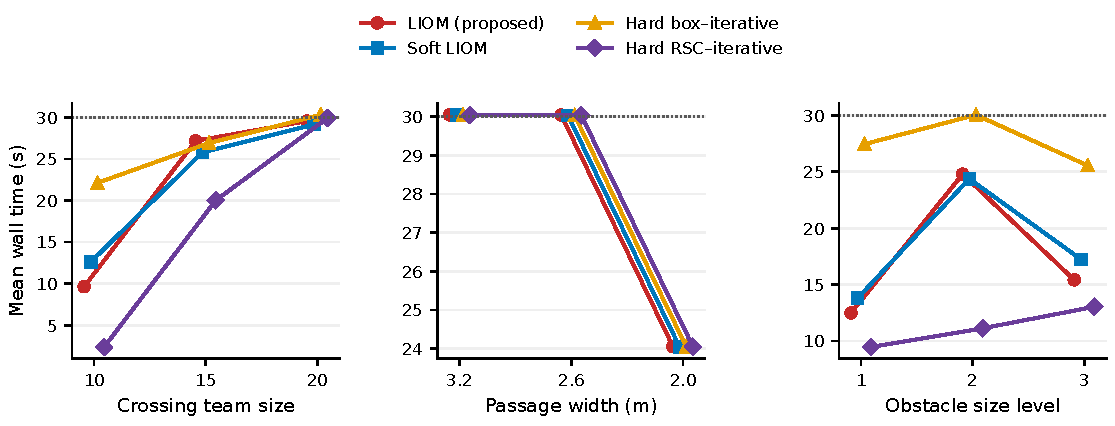
\includegraphics[width=\fulllength]{figures_revision/physical_congestion.pdf}
\caption{Computation under physical congestion with fixed corridor-growth settings. Panels vary crossing-team size, passage width, and obstacle size. Symbols distinguish methods in grayscale, and all attempts enter each mean.\label{fig:physical}}
\end{adjustwidth}\end{figure}

The grid study combines $N\in\{5,10,15,20\}$ and $K\in\{30,60,90\}$ with two predetermined realizations per combination. This separates team growth from discretization changes. Figure~\ref{fig:scaling} relates measured computation to problem size and shows the stage breakdown. The number of pair restrictions can decrease substantially after spatial-box screening, while complete-interval validation still checks all pairs.
\begin{table}[htbp]
\begin{adjustwidth}{-\extralength}{0cm}
\caption{Team/grid scaling over two realizations per setting. Mean wall times include all attempts. Variables and rows are the proposed method's mean maximum dimensions; coupling varies with the spatial boxes.\label{tab:scaling-new}}
\centering\small
\begin{tabular}{lrrrrr}\toprule
$N$ & $K$ & LIOM wall (s) & Hard RSC wall (s) & Variables & Rows\\\midrule
5 & 30 & 0.16 & 0.13 & 870 & 7,710\\
5 & 60 & 0.21 & 0.18 & 1,770 & 15,497\\
5 & 90 & 0.46 & 0.44 & 2,670 & 23,285\\
10 & 30 & 21.82 & 9.92 & 2,653 & 19,641\\
10 & 60 & 1.01 & 1.01 & 3,540 & 32,012\\
10 & 90 & 11.13 & 3.66 & 7,759 & 57,477\\
15 & 30 & 30.05 & 25.00 & 4,770 & 34,200\\
15 & 60 & 22.38 & 5.95 & 9,249 & 66,477\\
15 & 90 & 25.88 & 27.80 & 13,698 & 98,568\\
20 & 30 & 30.04 & 30.02 & 7,476 & 52,299\\
20 & 60 & 26.98 & 21.87 & 14,379 & 100,914\\
20 & 90 & 21.75 & 30.06 & 21,233 & 149,238\\
\bottomrule\end{tabular}
\end{adjustwidth}
\end{table}

\begin{figure}[htbp]
\begin{adjustwidth}{-\extralength}{0cm}\centering
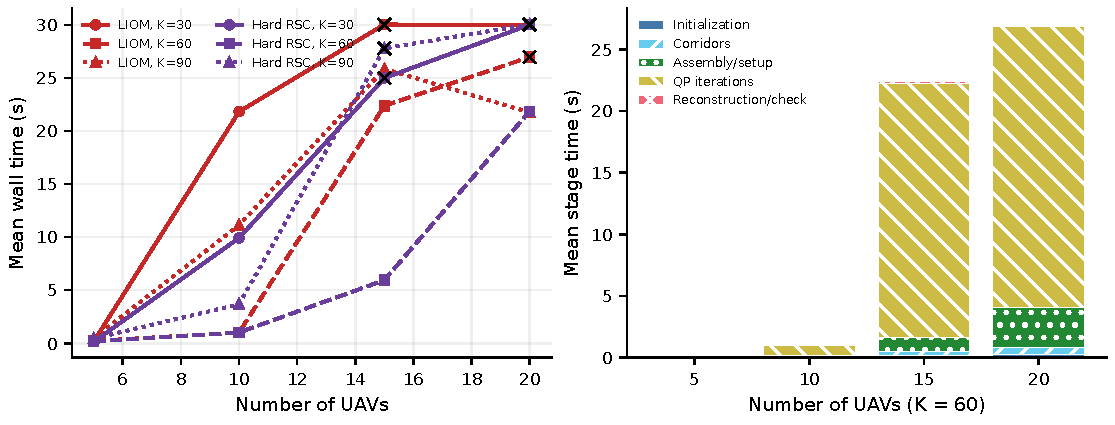
\includegraphics[width=\fulllength]{figures_revision/scaling_breakdown.pdf}
\caption{Team/grid scaling and planning-time components. Crosses mark team--grid groups with at least one attempt not accepted within 30 s. The stage breakdown includes initialization, corridor construction, assembly and solver setup, QP iterations, and final checking.\label{fig:scaling}}
\end{adjustwidth}\end{figure}
The reduced-horizon study varies $T_f$ from 8 to 12 s on six fixed geometries with unchanged corridor-growth caps. The accompanying records contain the candidate checks, outer rounds, and stopping outcomes for every method and setting.


\subsection{Mechanism and Parameter Studies}
A separate entry-budget study varies the initial hard-QP allowance between 1, 3, and 5 s on the ten tasks used in Table~\ref{tab:external}. All other settings and the total planning budget remain fixed. Table~\ref{tab:entry-budget} reports the complete runs, including recovery after the entry solve. In C29, the 3 s entry returns directly and reduces total time from 19.27 to 3.63 s and QP calls from five to one. The 3 s setting also returns accepted 15- and 20-UAV motions within budget in this study. Giving the initial hard problem 5 s reduces the time available for subsequent recovery: Winding A then returns its accepted motion after the total budget. The 3 s allowance offers a useful compromise and is recommended for new runs. The earlier benchmark and scaling records retain their original 1 s allowance; their recorded times are unchanged.
\begin{table}[htbp]
\begin{adjustwidth}{-\extralength}{0cm}
\caption{Hard-entry budget ablation. Each cell gives total planning time in seconds and QP calls. All three settings share the recorded reference and a 30 s total budget, with rotated execution order. $\times$ marks no accepted motion and $\dagger$ marks late acceptance.\label{tab:entry-budget}}
\small\begin{tabularx}{\fulllength}{Yrrr}\toprule
Task & 1 s entry: time / QPs & \textbf{3 s entry: time / QPs} & 5 s entry: time / QPs\\\midrule
C01 & 1.75 / 1 & 0.95 / 1 & 0.88 / 1\\
C03 & 1.35 / 1 & 1.44 / 1 & 1.46 / 1\\
C05 & 2.84 / 1 & 2.91 / 1 & 2.89 / 1\\
C25 & 1.20 / 1 & 1.18 / 1 & 1.17 / 1\\
C27 & 24.08 / 6 & 26.15 / 6 & 28.29 / 6\\
C29 & 19.27 / 5 & 3.63 / 1 & 3.65 / 1\\
Winding A & 28.70 / 5 & 30.00 / 5 & 31.33$^{\dagger}$ / 5\\
Winding B & 30.48$^{\dagger}$ / 6 & $\times$\,30.07 / 5 & $\times$\,30.04 / 5\\
15-UAV & $\times$\,30.08 / 7 & 29.09 / 6 & $\times$\,30.66 / 6\\
20-UAV & 28.37 / 6 & 27.04 / 6 & 30.35$^{\dagger}$ / 6\\
\bottomrule\end{tabularx}
\end{adjustwidth}\end{table}


\begin{table}[htbp]
\caption{Soft-loop acceptance feedback and motion-envelope studies on six scenes. Feedback combines tolerance tightening with an exact-kinematics finish; its components are evaluated jointly.\label{tab:mechanism-new}}
\centering\small
\begin{tabular}{lrr}\toprule
Variant & Wall (s) & QP calls\\\midrule
Aggregate, no feedback & 1.12 & 1.33\\
Aggregate + feedback & 1.12 & 1.33\\
Normalized, no feedback & 1.07 & 1.17\\
Normalized + feedback & 1.07 & 1.17\\
cube motion envelope & 1.03 & 1.33\\
hull14 motion envelope & 1.08 & 1.17\\
hull26 motion envelope & 1.16 & 1.17\\
\bottomrule\end{tabular}
\end{table}
The hard-iterative comparison holds reconstruction opportunities fixed. The hard-entry ablation compares proposed LIOM with Soft LIOM. The acceptance-feedback study examines how rejected reconstructed motions affect subsequent computation; it also records rejection reasons and additional exact-QP calls.



% BEGIN FEEDBACK COUNTS
The six anchor tasks are accepted under all four recovery-criterion/feedback variants. Across the eight frozen suites, 23 reconstructed soft candidates fail a physical check, in 19 attempts; 15 of those attempts later return an accepted motion within budget. The exact-finishing branch returns 9 accepted motions. Across the 1,212 attempts in the eight frozen suites, four initialization failures concern one physical scene evaluated by four methods. The static-guide fallback follows 93 SFM simulation timeouts; no scalar-timing failure is recorded in these suites. Counts refer to attempted executions, including timing repetitions.
% END FEEDBACK COUNTS

\begin{table}[htbp]
\begin{adjustwidth}{-\extralength}{0cm}
\caption{Reference geometry and later guide availability crossed on six anchor scenes. Mean times and rounds include all attempts; task-level outcomes accompany the data.\label{tab:initialization-new}}
\centering\small
\begin{tabular}{lrrr}\toprule
Reference & Relocation guide & Wall (s) & Rounds\\\midrule
SFM + guide fallback & False & 1.09 & 1.17\\
SFM + guide fallback & True & 1.08 & 1.17\\
Straight & False & 18.76 & 9.00\\
Straight & True & 17.98 & 7.17\\
Static guide & False & 17.95 & 7.17\\
Static guide & True & 17.93 & 7.17\\
\bottomrule\end{tabular}
\end{adjustwidth}
\end{table}

\begin{table}[htbp]
\begin{adjustwidth}{-\extralength}{0cm}
\caption{One-factor sensitivity on six anchor scenes, all accepted at the tested settings. Columns give mean wall time after halving or doubling one parameter; the last row uses the stated growth factors. Nominal time is 1.07 s.\label{tab:sensitivity-new}}
\centering\small
\begin{tabular}{lrr}\toprule
Changed factor & Lower value: wall (s) & Higher value: wall (s)\\\midrule
Control effort $w_a$ & 1.00 & 1.08\\
Initial defect penalty & 1.08 & 1.01\\
Initial slack penalty & 1.07 & 1.08\\
Defect penalty cap & 1.08 & 1.08\\
Slack penalty cap & 1.07 & 1.08\\
Normalized defect tolerance & 1.07 & 1.07\\
Mean slack tolerance & 1.07 & 1.07\\
Spatial growth cap & 1.06 & 1.10\\
Relative growth cap & 2.51 & 1.09\\
SFM repulsion & 1.08 & 1.09\\
SFM decay length & 1.14 & 3.60\\
SFM look-ahead & 6.06 & 1.08\\
SFM response time & 1.10 & 1.08\\
SFM tangential fraction & 1.16 & 1.07\\
Candidate row tolerance & 1.08 & 1.08\\
Penalty growth (1.5 / 5) & 1.08 & 1.08\\
\bottomrule\end{tabular}
\end{adjustwidth}
\end{table}

\begin{table}[htbp]
\begin{adjustwidth}{-\extralength}{0cm}
\caption{OSQP audit on identical matrices from three anchor scenes. Readiness stopping is compared with ordinary termination at two tolerances. The feasible-column criterion is maximum linear-row violation $\leq10^{-3}$; full trajectories still require physical acceptance.\label{tab:solver-new}}
\centering\small
\begin{tabular}{lrrrrr}\toprule
QP & Termination & Row test & Max. violation & Time (s) & Iterations\\\midrule
soft & Readiness & 3/3 & 5.2e-05 & 1.94 & 6,833\\
soft & Standard ($10^{-6}$) & 3/3 & 5.2e-05 & 1.96 & 6,833\\
soft & Standard ($10^{-7}$) & 3/3 & 1.4e-05 & 6.40 & 20,000\\
hard & Readiness & 2/3 & 1.5e+10 & 1.64 & 5,808\\
hard & Standard ($10^{-6}$) & 2/3 & 1.5e+10 & 4.10 & 13,767\\
hard & Standard ($10^{-7}$) & 2/3 & 1.5e+10 & 4.93 & 16,308\\
rsc & Readiness & 3/3 & 8.7e-04 & 0.45 & 1,400\\
rsc & Standard ($10^{-6}$) & 3/3 & 1.6e-15 & 1.37 & 4,733\\
rsc & Standard ($10^{-7}$) & 3/3 & 1.6e-15 & 2.80 & 9,283\\
\bottomrule\end{tabular}
\end{adjustwidth}
\end{table}

The initializer study crosses SFM, straight geometry, and static-guide geometry with guide availability during later relocation. It separates reference construction from the use of a guide after the initial solve. Penalty, tolerance, corridor-size, and SFM sensitivity tests change one factor at a time on six anchor tasks. Corridor-size changes are treated as a numerical sensitivity study; the physical-congestion comparisons retain the nominal limits. The motion-envelope study compares the original cube with 14- and 26-vertex inner approximations. The acceptance study compares aggregate and normalized recovery criteria, with and without acceptance feedback.

\FloatBarrier
\subsection{Rigid-Body Tracking in a Physics Simulator}
\label{sec:tracking}
After centralized planning, each UAV receives its time-indexed position, velocity, and acceleration reference. A shared execution clock preserves their temporal coordination. Individual feedback controllers track these references; all inter-UAV decisions have already been coupled in the centralized solve. This architecture assumes known initial states and a common static map.

\begin{figure}[!htbp]
\begin{adjustwidth}{-\extralength}{0cm}\centering
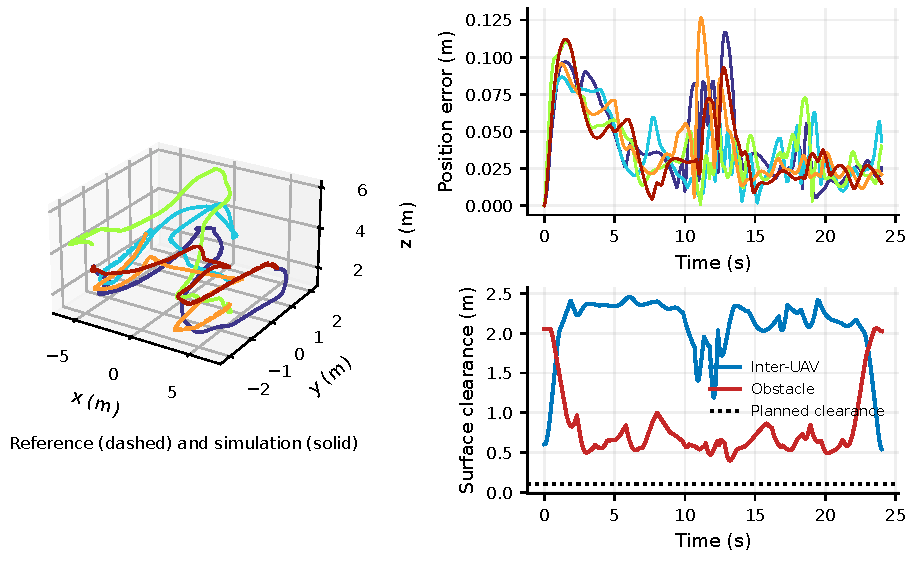
\includegraphics[width=\fulllength]{figures_revision/tracking.pdf}
\caption{Rigid-body execution of a planned cooperative motion: reference and simulated positions, tracking error, and surface clearance. Simulation measurements are sampled at the physics integration rate.\label{fig:tracking}}
\end{adjustwidth}\end{figure}

MuJoCo~\cite{todorov2012mujoco} provides six-degree-of-freedom rigid-body dynamics, gravity, bounded rotor actuation, motor lag, and contact detection. The generic quadrotor has mass 1 kg, inertia $\operatorname{diag}(0.006,0.006,0.010)$ kg m$^2$, rotor coordinates $(\pm0.14,\pm0.14,0)$ m, and a 5 N force limit per rotor. Motor lag is 0.02 s and the integration step is 0.002 s. Position/velocity feedback and a rotation-matrix attitude controller generate four rotor-force commands. The perturbed condition increases mass by 10\%, motor lag by 50\%, and adds sinusoidal wind force with 0.15 N amplitude per coordinate. Controller settings are fixed across the evaluated scenes.

The simulator evaluates all accepted proposed-method motions from the first main-benchmark repetition and predetermined accepted larger-team and winding-recovery examples. The same controller is used in the nominal and perturbed conditions. Table~\ref{tab:tracking-new} reports position error, terminal accuracy at the specified completion time, separation, and contact outcomes. Full time histories, simulator models, and settings accompany the results.

\begin{table}[htbp]
\begin{adjustwidth}{-\extralength}{0cm}
\caption{MuJoCo tracking over the prescribed flight interval. Terminal error is measured at $T_f$, before the separately logged settling interval. Clearance is center distance minus two planning radii.\label{tab:tracking-new}}
\centering\small
\begin{tabular}{lrrrrrr}\toprule
Condition & Motions & Max. error (m) & Mean RMS (m) & Terminal (m) & Pair gap (m) & Contact runs\\\midrule
Nominal & 35 & 0.132 & 0.017 & 0.105 & 0.504 & 0\\
Perturbed & 35 & 0.139 & 0.057 & 0.121 & 0.469 & 0\\
\bottomrule\end{tabular}
\end{adjustwidth}
\end{table}


The closed-loop simulations assess how the planned motions are tracked under rotor-force limits, motor lag, and disturbances. Tracking errors and surface clearances characterize execution by the feedback controller. The planning model and continuous-interval checks supply the corresponding reference-motion assessment.
